Last time, we defined the Cartan matrix $A^{ij}$ and said that for simple Lie algebras, we have some strong constraints on the possible Cartan matrices. They are as follows:
\begin{enumerate}
    \item $A^{ii}=2$
    \item $A^{ij}=0\iff A^{ji}=0$
    \item $A^{ij}\in \ZZ_{\leq 0}$ for $i\neq j$
    \item $\det A >0$
    \item $A$ irreducible (cannot be written in block diagonal form).
\end{enumerate}

Moreover, our labeling of the simple roots as $i=1,\ldots,r$ is totally arbitrary, so we would like to avoid overcounting and treat two Cartan matrices as equivalent up to a relabeling of the roots. We do so by using \term{Dynkin diagrams}.

The rules for drawing Dynkin diagrams are as follows.
\begin{itemize}
    \item Draw a node $O$ for each simple root $i=1,\ldots,r$.
    \item Join nodes corresponding to simple roots $\alpha_{(i)}$ and $\alpha_{(j)}$ such that $\max\set{|A^{ij}|,|A^{ji}|}\in \set{0,1,2,3}$.
    \item If the roots have different lengths, draw an arrow from the longer root to the shorter one.
\end{itemize}

If we categorize the kind of simple Lie algebras we can draw up to isomorphism of their Dynkin diagrams, we find that there are 4 infinite families of Lie algebras, plus five exceptional cases.
\begin{itemize}
    \item $A_n$ (e.g. $L_\CC(SU(n+1))$)
    \item $B_n$ (e.g. $L_\CC(SO(2n+1))$)
    \item $C_n$ (e.g. $L_\CC(SP(2n))$)
    \item $D_n$ (e.g. $L_\CC(SO(2n))$).
\end{itemize}
There are also the exceptional cases $E_6,E_7,E_8,F_4,G_2$, depicted in Fig. \ref{fig:dynkin2}.

\begin{figure}
    \centering
    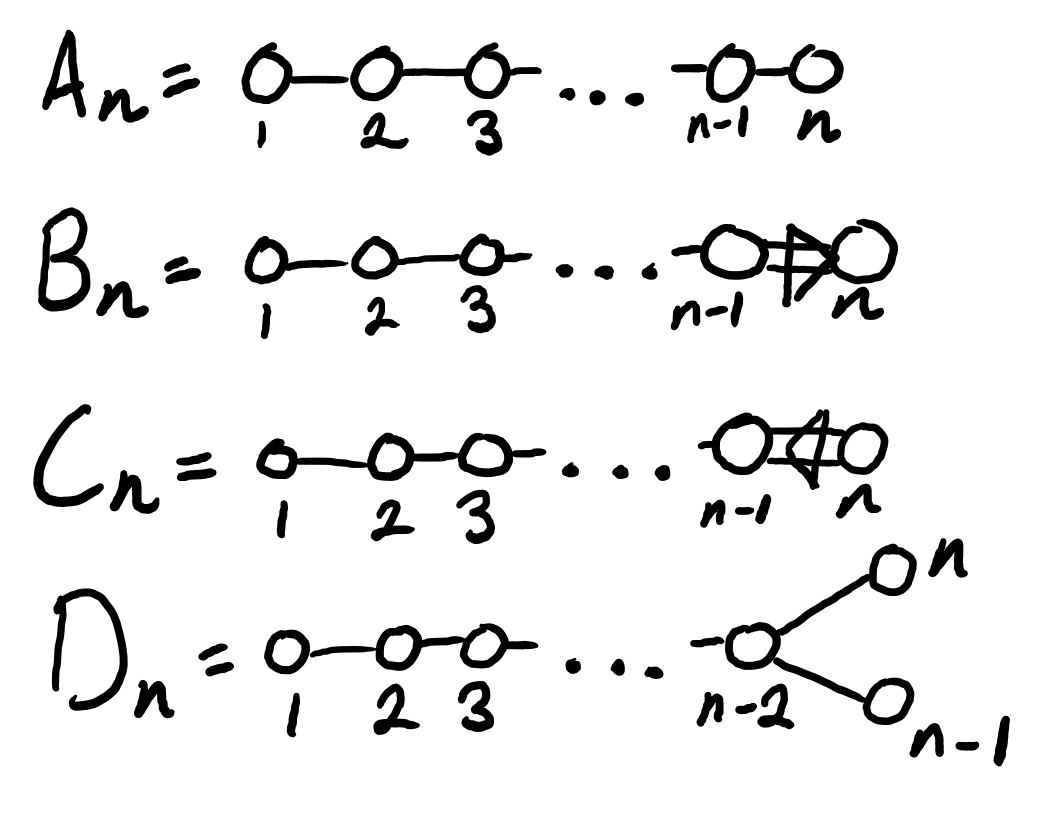
\includegraphics{2018/11/20181117_cartan1.png}
    \caption{The Dynkin diagrams for the four infinite families of Lie algebras: $A_n,B_n,C_n,$ and $D_n$. By considering cases for small $n$, we can recognize immediately from the diagrams that some common Lie algebras are isomorphic. For instance, $B_2$ and $C_2$ have two nodes connected by two lines with an arrow, so $B_2\approx C_2 \approx L_\CC(SO(5)).$}
    \label{fig:dynkin1}
\end{figure}

\begin{figure}
    \centering
    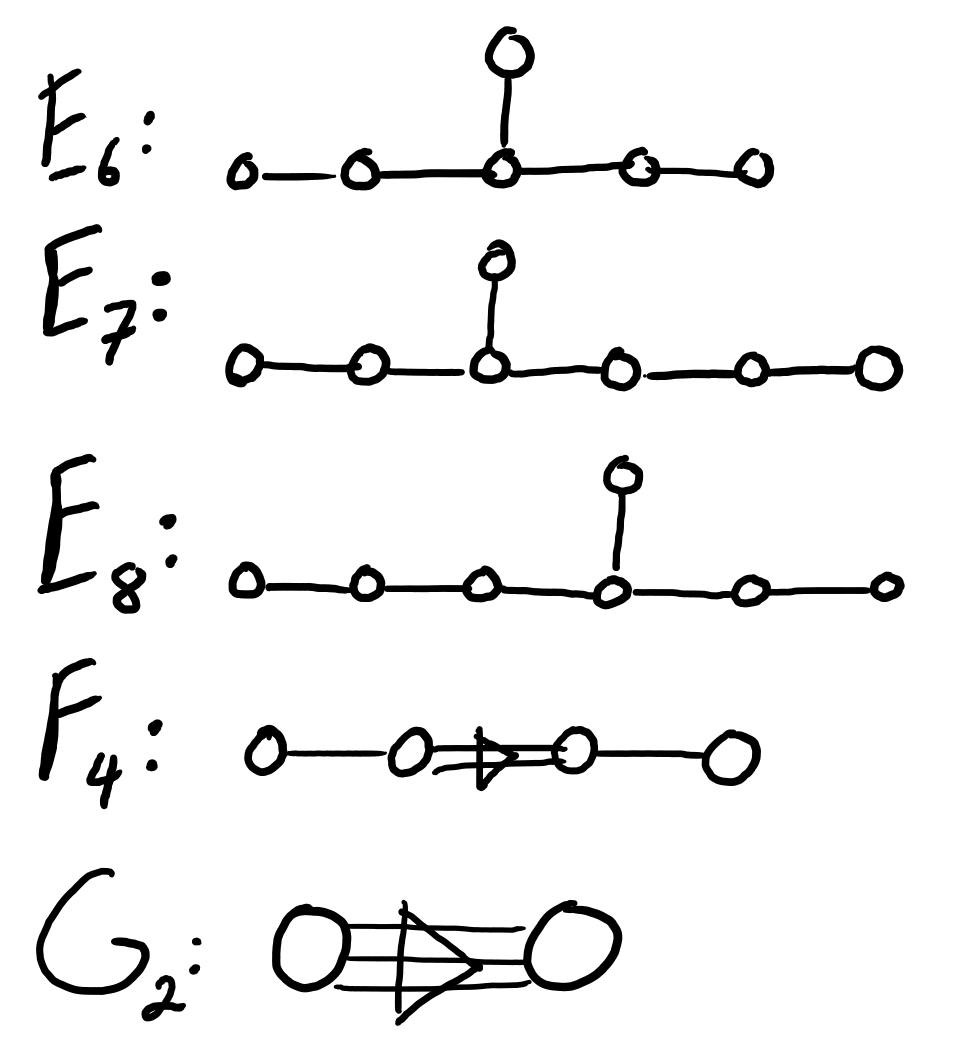
\includegraphics{2018/11/20181117_cartan2.png}
    \caption{The Dynkin diagrams for the five exceptional Lie algebras: $E_6,E_7,E_8,F_4,$ and $G_2$.}
    \label{fig:dynkin2}
\end{figure}

Note that for $n=1$, we have $A_1=B_1=C_1=L_\CC(SU(2))$. These are diagrams with a single isolated node. Therefore in terms of the actual Lie algebras, $$L_\CC(SU(2))=L_\CC(SO(3))=L_\CC(SP(2)).$$
For the $n=2$ case, we find that $A_2\approx L_\CC(SU(3))$ (two nodes connected by a single line). Meanwhile, $B_2\approx C_2 \approx L_\CC (SO(5))$ (two nodes connected by two lines and an arrow). From the diagrams, we observe immediately that $D_2=A_1 \oplus A_1$, since its diagram is just two disconnected nodes. Looking at the corresponding Lie algebras, we find that $L_\CC(SO(4))\simeq L_\CC(SU(2))\oplus L_\CC(SU(2)).$ We also see that $A_3=D_3$ (three nodes connected in a straight line), so we immediately recognize that $L_\CC(SU(4))\simeq L_\CC(SO(6)).$

Gauge theories are naturally associated to (simple) Lie algebras. Sometimes we restrict ourselves to diagrams with simple links, i.e. without arrows (the ``ADE classification''). Simple Lie algebras come up in string theory too-- Michael Green, a former Lucasian professor here at Cambridge, once proved that for heterotic string theory, the gauge group must either be $SO(32)$ or $E_8\times E_8$, or else the theory suffers a fatal anomaly. Thus even these exceptional cases turn out to be of interest in physics.

\subsection*{Reconstructing $\fg$ from $A$} The Cartan matrix contains a lot of information about the structure of the original Lie algebra.
$$A^{ij}=\frac{2(\a_{(i)},\a_{(j)})}{(\a_{(j)},\a_{(j)})}=\frac{2|\alpha_{(i)}|}{|\alpha_{(j)}|}\cos\phi_{ij}.$$
From here, one can work out the root strings. For example, if $\fg=A_2$, then the Cartan matrix is
$$A=\begin{pmatrix}
2&-1\\-1&2
\end{pmatrix}.$$
We learn that $\fg$ has two simple roots $\alpha,\beta \in \Phi$, such that
$$\frac{2(\alpha,\beta)}{(\alpha,\alpha)}=\frac{2(\beta,\alpha)}{(\beta,\beta)}=-1.$$
From this, we conclude that $|\alpha|=|\beta|$ and $\phi_{\alpha\beta}=2\pi/3$ since $2\cos\phi=-1$.
Since $\alpha,\beta\in \Phi_S$, we know that their difference is not a root, $\pm(\alpha-\beta)\notin \Phi.$ But the length of the $\alpha$ string through $\beta$ is
$l_{\alpha,\beta}=1-\frac{(\a,\beta)}{(\a,\a)}=+2$ and a similar calculation yields $l_{\beta,\alpha}=2$. Therefore since the root strings are
$$\beta+n\alpha, \alpha+\tilde n\beta \in \Phi$$
with $n,\tilde n \in \ZZ$, it must be that $n,\tilde n\in \set{0,1}.$ We conclude that the roots are
$$\alpha,\beta,\alpha+\beta\in \Phi$$
and also their negatives,
$$-\alpha,-\beta,-\alpha-\beta\in \Phi.$$
Fortunately, the counting works out. For $A_2\approx L_\CC(SU(3)),$ we know that the dimension is $D=8$ and the rank is $r=2$, so the number of step generators (and therefore the number of roots) we expect is indeed 6.

Moreover we can now express a general positive root $\alpha \in \Phi_+$ in the basis of the simple roots,
$$\alpha=\sum_{i=1}^r n_i \alpha_{(i)}, n_i \geq 0.$$
We say that the \term{height} of a root $\alpha$ is then
$$t(\alpha)=\sum_{i=1}^r n_i.$$
%
To complete our results, we see that the root system of $A_2$ is
$$\Phi=\set{\pm \a,\pm \beta,\pm(\alpha+\beta)}.$$
We also compute the inner product $$(\alpha+\beta,\alpha+\beta)=(\alpha,\alpha)+(\beta,\beta)+2(\alpha,\beta)=(\alpha,\alpha)[1+1-1]=(\alpha,\alpha).$$
Thus one can draw a diagram of the roots, as seen in Fig. \ref{fig:rootgeometry}.
\begin{figure}
    \centering
    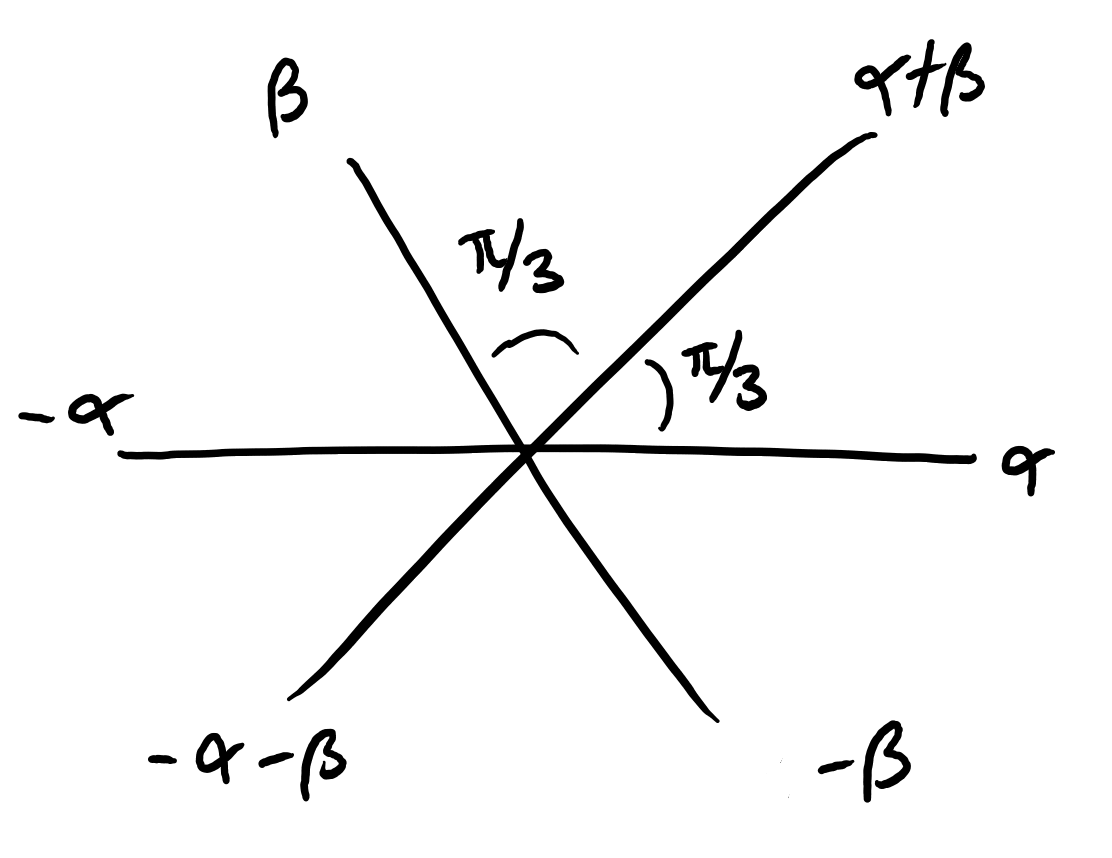
\includegraphics{2018/11/20181117_rootgeometry.png}
    \caption{The roots of the Lie algebra $\fg=A_2$. There are two simple roots, $\alpha$ and $\beta$, and they are separated by an angle of $\pi/6$. Based on the form of the Cartan matrix, we can take linear combinations and compute their inner products to see the geometric structure of the dual space $\fh^*$.}
    \label{fig:rootgeometry}
\end{figure}

Now let $R$ be a representation of a Lie algebra $\fg$ of dimension $N$. Recall that representations are maps which preserve the brackets in the original Lie algebra. In particular, the elements of the Cartan subalgebra $H^i\mapsto R(H^i)$ must have representations, as well as the step generators $E^\alpha \mapsto R(E^\alpha) \in \text{Mat}_N(\CC)$.

By the defining property of the $H^i$, it must be that $R(H^i)$ are diagonalizable, $i=1,\ldots,r$. Since brackets are preserved,
$$[R(H^i),R(H^j)]=R([H^i,H^j])=0\quad \forall i,j,$$
which means that the matrices $\set{R(H^i)}$ are \emph{simultaneously} diagonalizable. It follows that the representation space $V\simeq \CC^N$ is spanned by the simultaneous eigenvectors of $\set{R(H^i)}$.

We can think of the full representation space as the direct sum of the eigenspaces spanned by the eigenvalues,
$$V=\bigoplus_{\lambda\in S_0} V_\lambda.$$
For $v\in V_\lambda$, we have
$R(H^i)v=\lambda^i v, \lambda^i \in \CC.$
The eigenvalue $\lambda \in \fh^*$ is a weight of the representation $R$, and collectively they form a weight set $S_R.$